\section{Overview of KL3M Collection Process}
In developing the Kelvin Legal Large Langugage Model (KL3M), we sought to collect and curate a large body of information which was free from the specter of copyright infringement. As opposed to broad data collected from the internet writ large, we sought to identify sources of high quality information, free from copyright concerns that were reasonably available online.  Governmental data, thus currently represents the vast majority of data within the Kelvin Legal Large Language Model (KL3M) dataset. As an output of the growth of the modern regulatory state,\cite{katz2020complex}\cite{coupette2021measuring} various components of government produce very large bodies of relatively high-quality information content.  In addition, various legal and regulatory processes require individuals and organizations to draft and submit various forms of information to government officials, often with guidance and oversight by lawyers, accountants and other professionals.  
%This led us to primarily focus on information produced by or otherwise made available by government(s) as among other things such data is much higher quality than typical internet data.  

While the substantive quality of many forms of governmental data is quite high, the organization and accessibility of such information is not always nearly as strong.  Although governmental and other related data has slowly made it way into the digital world, the mere digitization of governmental information or work product has not always allowed the public to obtain the crucial information they need.  Poorly designed websites, a lack user-friendly navigation and outdated and inconsistent digital platforms are just some of the challenges faced by individuals engaging with public sector information systems.  We faced these very challenges in collecting and curating the KL3M dataset. Although much of this data is theoretically accessible, it is often stored in various inconsistent formats which make cross-functional access very difficult even in discrete amounts (let alone at scale). 

In this section, we begin by discussing trends in modeling building while providing some exemplars of the wide-ranging content contained within the KL3M dataset.  Next, we detail our efforts to collect, pre-process and organize this vast and diverse corpora.  Finally, we provide a high level overview of the distribution of sources contained within the current version of the Kelvin Legal Large Language Model (KL3M) dataset. 
  
\subsection{Breadth and Quality of Tokens Might Be What You Need}
One challenge in building modern language models is to have both scale and a diversity of pre-training information content to cover the broad conceptual space of potential user queries.  Users might want to ask a model to explain a scientific question, determine how best to cook a particular recipe, look to draft some long-form prose or perhaps even ask questions about how to sublease their apartment.  The prevailing approach to cover the broad conceptual space of potential user queries is simply to scale models to increasing large scales.\cite{kaplan2020scaling}  ``Chinchilla'' and other related scaling laws have encouraged model builders to pre-train on the maximal amount of available pretraining data.\cite{hoffmann2022training}\cite{pearce2024reconciling}.  As such, most developments in LLMs have been focused on the use of various collections of internet and so called ``publicly available'' data to build larger and larger language models. 

Undoubtably, the sheer power of scale has delivered some fairly remarkable results. Engineering, however, is not only about performance, it is also about cost.\cite{Krishna2025}  Thus, an alternative strain of work has focused upon how to cost effectively train models using distillation and other related techniques.\cite{guo2025deepseek}\cite{zhang2024tinyllama}\cite{javaheripi2023phi} The scaling laws upon which the field was once fixated have arguably given way to a more nuanced perspective where token diversity, token quality and test time inference scaling are also an important part of the overall calculus.\cite{snell2024scaling}\cite{yu2024makes}  

\subsection{The Incredible Expanse of Government Work Product}
Legal and regulatory processes implicate a wide variety of pursuits and fields of human endeavour.  Thus, taken as a whole, the work product of governments and governmental processes covers a significant amount of intellectual territory.  While certainly not covering every topic that a user might find interesting, information from governments covers a surprising amount of the broader conceptual space.  Laws, regulations, scientific reports, food safety bulletins, environmental impact assessments, public health guidelines, statistical reports, press releases, disaster preparedness plans, government contracts and certain private contracts, judicial opinions, public commentary, military directives, food and drug recalls, transportation safety reports, economic forecasts, patent filings, congressional testimony, securities filings, census data reports are just some examples of the outputs associated with the governmental work product and governmental processes.  

KL3M features a wide variety of question and answer pairs, professional dialogues, formal definitions of key terminology and parallel assessment documents in multiple languages.  It is quite difficult to fully characterize the incredible expanse of topics and materials contained therein.  Appendix I highlights the KL3M Data Gallery, an online exploration tool which allows users to review millions of sample documents drawn from the broader KL3M dataset.  However, consider Figure \ref{fig:KL3MImages} which offers just a few selected examples that are exemplars of the broader set of data contained in KL3M.  Across the four examples, we observe a wide range of topics from turducken food handling, micronutrient testing in vitamins and carotenoids, mineral resources of the Owyhee River Canyon in Idaho and an analysis of the change in input impedance for electrically short dipole antennas.  Agencies represented such as the United States Department of Agriculture, NIST, Department of Commerce and the Department of Interior are just a small subset of the total agencies producing government work product on a daily basis.

\begin{figure}[H]
\centering
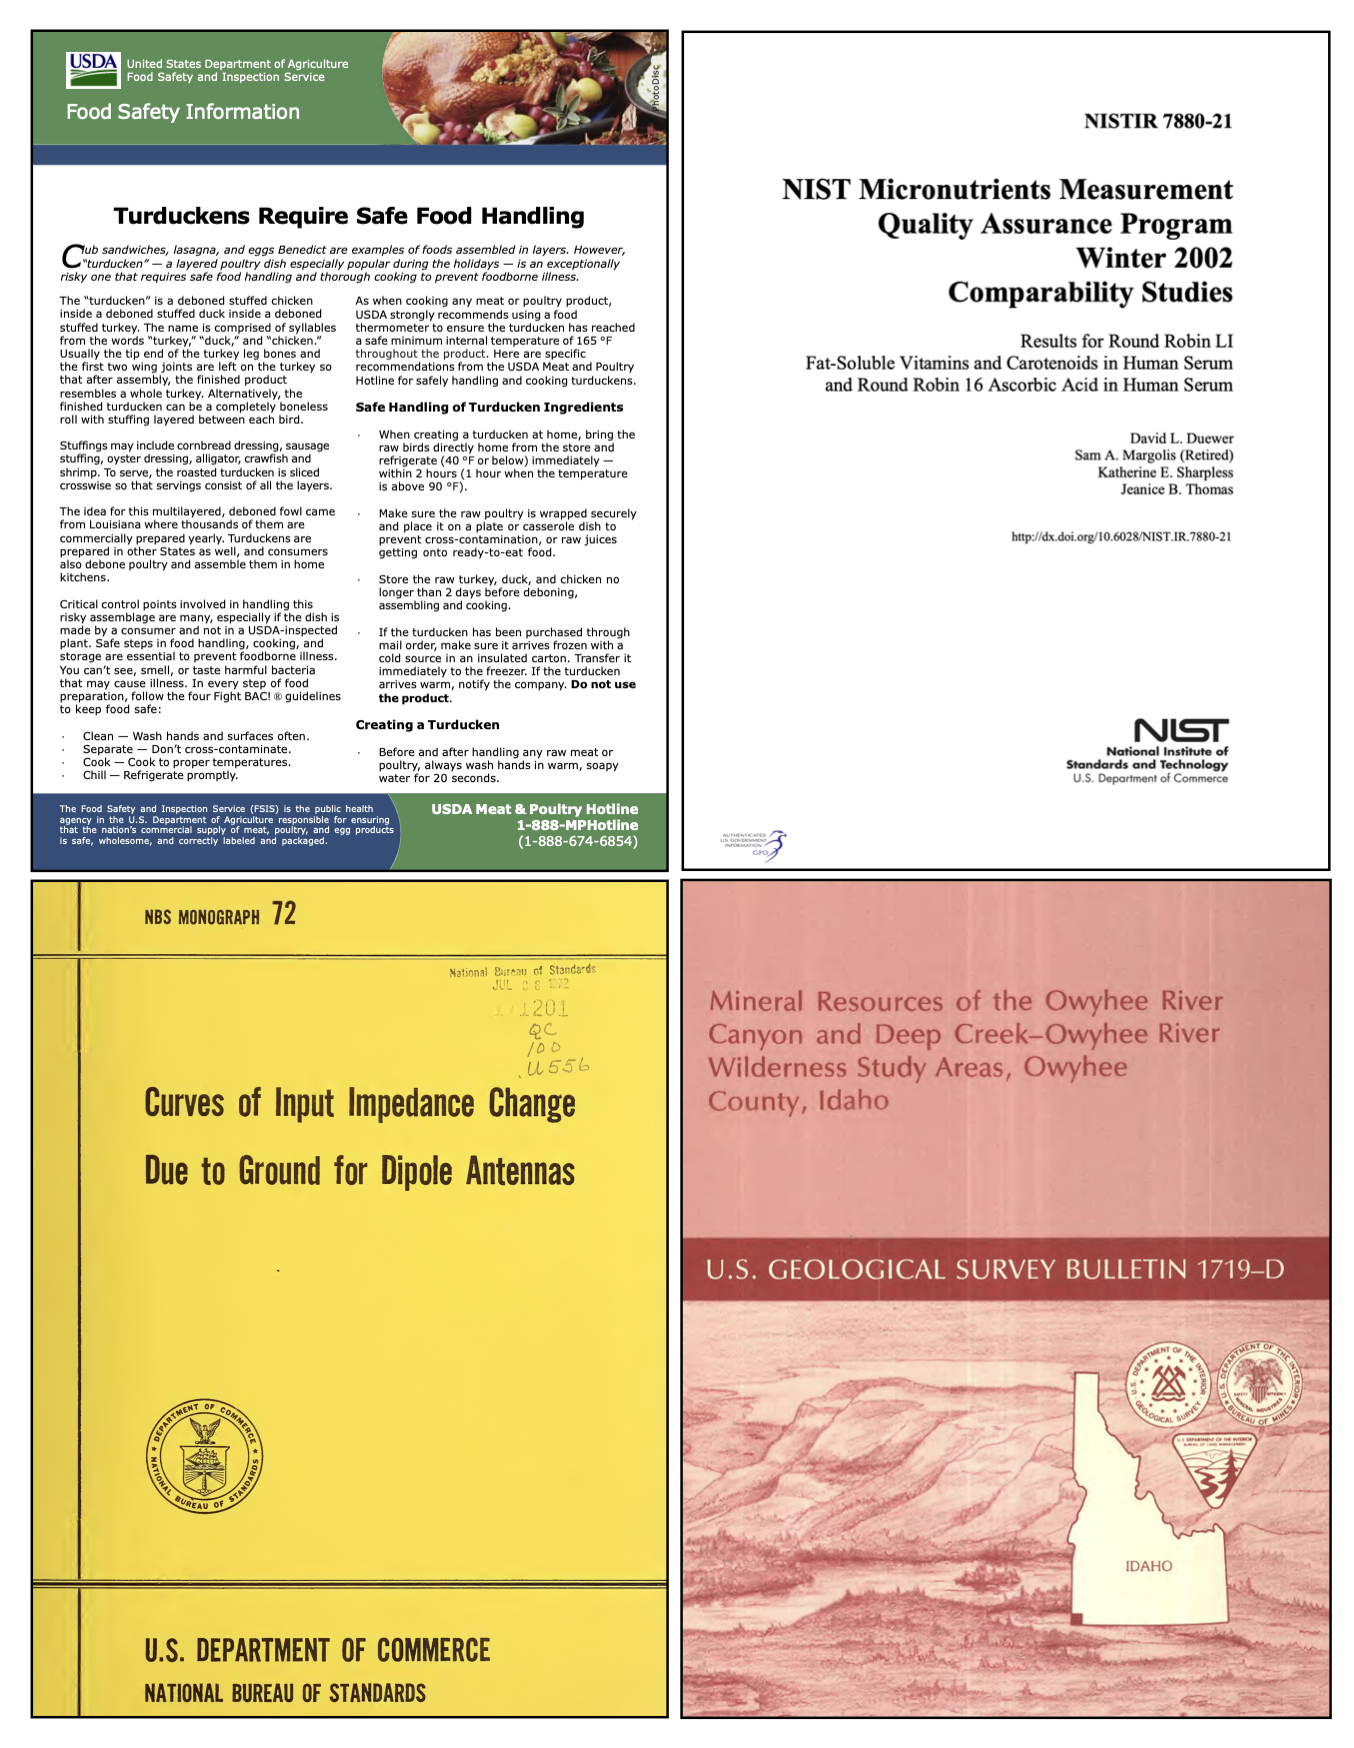
\includegraphics[width=95mm]{KL3MImages.png}
\caption{\centering{Samples of Content from the KL3M Dataset}}
\label{fig:KL3MImages}
\end{figure}

\subsection{The Collection \& Pre-Processing Data Pipeline for KL3M}
Working with the vast array of document types such as those displayed in Figure \ref{fig:KL3MImages} is a challenging proposition.  To do so effectively at scale, we developed a pre-processing pipeline designed to engage with the real-life challenges associated with the unstructured, inconsistent and complex forms of documents across the various information systems with which we engaged.  Thus, in addition to the KL3M dataset, we are also releasing all of the tooling and libraries leveraged across the KL3M Pre-Processing pipeline as it is our hope that others might adapt this work in order to build parallel corpora in other jurisdictions.   

\begin{figure}[h!]
\centering
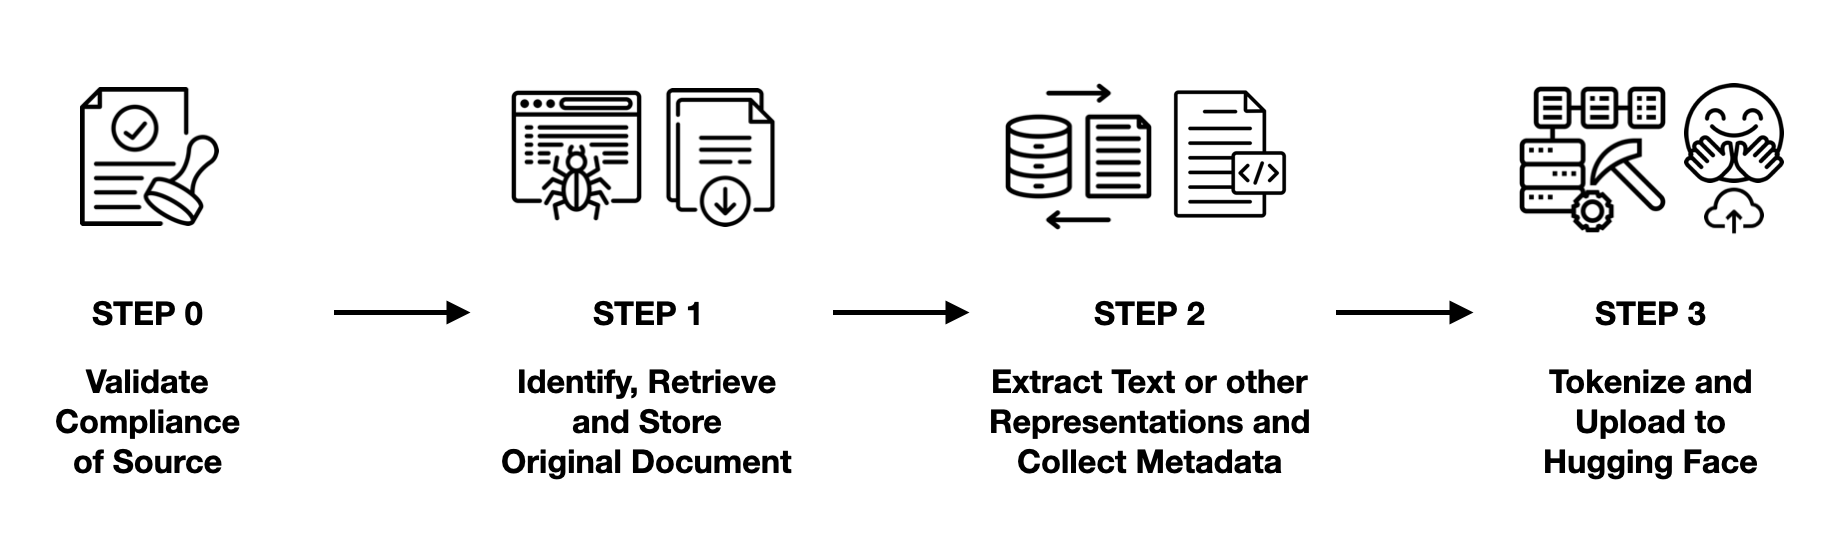
\includegraphics[width=150mm]{PreProcessing.png}
\caption{\centering{{Overview of the Pre-Processing Pipeline} - (icons via Flaticon)}}
\label{fig:preprocessing}
\end{figure}


Figure \ref{fig:preprocessing} provides a high-level overview of our pre-processing pipeline.  Building from our copyright filtration process described in Figure \ref{fig:CopyrightFlowchart}, we begin by identifying a potential source of useful content.  Next, we must determine whether that candidate source complies with our requirements. Thus, \textit{Step 0} is high level recitation of the process described in Figure \ref{fig:CopyrightFlowchart}.  Having then identified and validated compliance of the source material, we next proceed to \textit{Step 1} of Figure \ref{fig:preprocessing} where we retrieve and retain the original source material for provenance purposes.\footnote{This ability to demonstrate original source provenance was critical in obtaining the \textit{Fairly Trained} Certification described in Section 3.2.}  

In \textit{Step 2}, we develop an alternative representation of the documents which varies depending upon the nature of the original source.  Our ideal path is to build an alternative representation of all source materials in Markdown \cite{mailund2019beginner} while also retaining the original source material in parallel.  However, this is not always possible given the nature of the original source.  Finally, in \textit{Step 2} were also collect and store \textit{Dublin Core Metadata} for all source material.  

In \textit{Step 3}, we tokenize all objects using a custom tokenizer developed specifically for this task.  The KL3M tokenizer has several specific elements that makes it unique \color{red}\textbf{[MIKE ADD HERE 2-3 sentences]} \color{black}  Finally, we upload the tokenized document to their respective folder on \textit{Hugging Face}.\footnote{The KL3M Data can be access here \url{https://huggingface.co/collections/alea-institute/kl3m-data-679f9db9b6fd93f91c3c633e}}

